\documentclass[12pt]{article}			% For LaTeX 2e
						% other documentclass options:
						% draft, fleqn, openbib, 12pt

\usepackage{graphicx}	 			% insert PostScript figures
\usepackage{caption}
\usepackage{subcaption}
\usepackage{wrapfig}
\usepackage{amsmath}
%% \usepackage{setspace}   % controllabel line spacing
%% If an increased spacing different from one-and-a-half or double spacing is
%% required then the spacing environment can be used.  The spacing environment 
%% takes one argument which is the baselinestretch to use,
%%         e.g., \begin{spacing}{2.5}  ...  \end{spacing}


% the following produces 1 inch margins all around with no header or footer
\topmargin	=10.mm		% beyond 25.mm
\oddsidemargin	=0.mm		% beyond 25.mm
\evensidemargin	=0.mm		% beyond 25.mm
\headheight	=0.mm
\headsep	=0.mm
\textheight	=220.mm
\textwidth	=165.mm
					% SOME USEFUL OPTIONS:
% \pagestyle{empty}			% no page numbers
 \parindent  15.mm			% indent paragraph by this much
 \parskip     2.mm			% space between paragraphs
% \mathindent 20.mm			% indent math equations by this much

\newcommand{\MyTabs}{ \hspace*{25.mm} \= \hspace*{25.mm} \= \hspace*{25.mm} \= \hspace*{25.mm} \= \hspace*{25.mm} \= \hspace*{25.mm} \kill }

\graphicspath{{../Figures/}{../data/:}}  % post-script figures here or in /.

					% Helps LaTeX put figures where YOU want
 \renewcommand{\topfraction}{0.9}	% 90% of page top can be a float
 \renewcommand{\bottomfraction}{0.9}	% 90% of page bottom can be a float
 \renewcommand{\textfraction}{0.1}	% only 10% of page must to be text

\linespread{1.2}
\alph{footnote}				% make title footnotes alpha-numeric

\begin{document}			% REQUIRED

\begin{center}
	{\LARGE \bf Framework}
\end{center}
This section intends to propose a framework for the Continuous Authentication system that has been described so far. It is an abstract definiton of the subsystems that are a part of this system and the interactions occurring amongst and inside them. A description of the whole system and its working will be followed by a detailed description of the subsystems.

The proposed system operates in two phases, as required, namely - Training and Continuous Authentication. For the system to be able to recognize a user via face recognition, the user's facial features have to be captured, during the account creation period, for training. Hence, the Training phase. Once the face recognition model has been retrained with a new user's facial features, the user can be recognized during and after log-in. Successful recognition implies the user is authenticated and logged-in. This is followed by continual verification of the user's Hard Biometric traits, which upon going beyond a given threshold of confidence level, moves onto the user's Soft Biometric traits. This shift reduces the computational load on the processor and also allows the user a higher degree of freedom in moving his/her face (as opposed to facing the camera). In our system, we take the user's clothing to be his/her Soft Biometric trait, which can be expected to stay constant during a session. As long as the Soft Biometric traits verification maintains a high confidence in the identity of the user, it continues. If it falls, Face Recognition kicks in to verify the user's identity. This continues till the session ends. During the session, if an imposter tries tailgating the authenticated user, the system enters into a lockdown mode. Upon return of the authentic user, the system performs a face recognition and automatically logs the user back in. The working of this system can be illustrated by the block diagram shown below. 

\begin{figure}[h!]
        \centering
        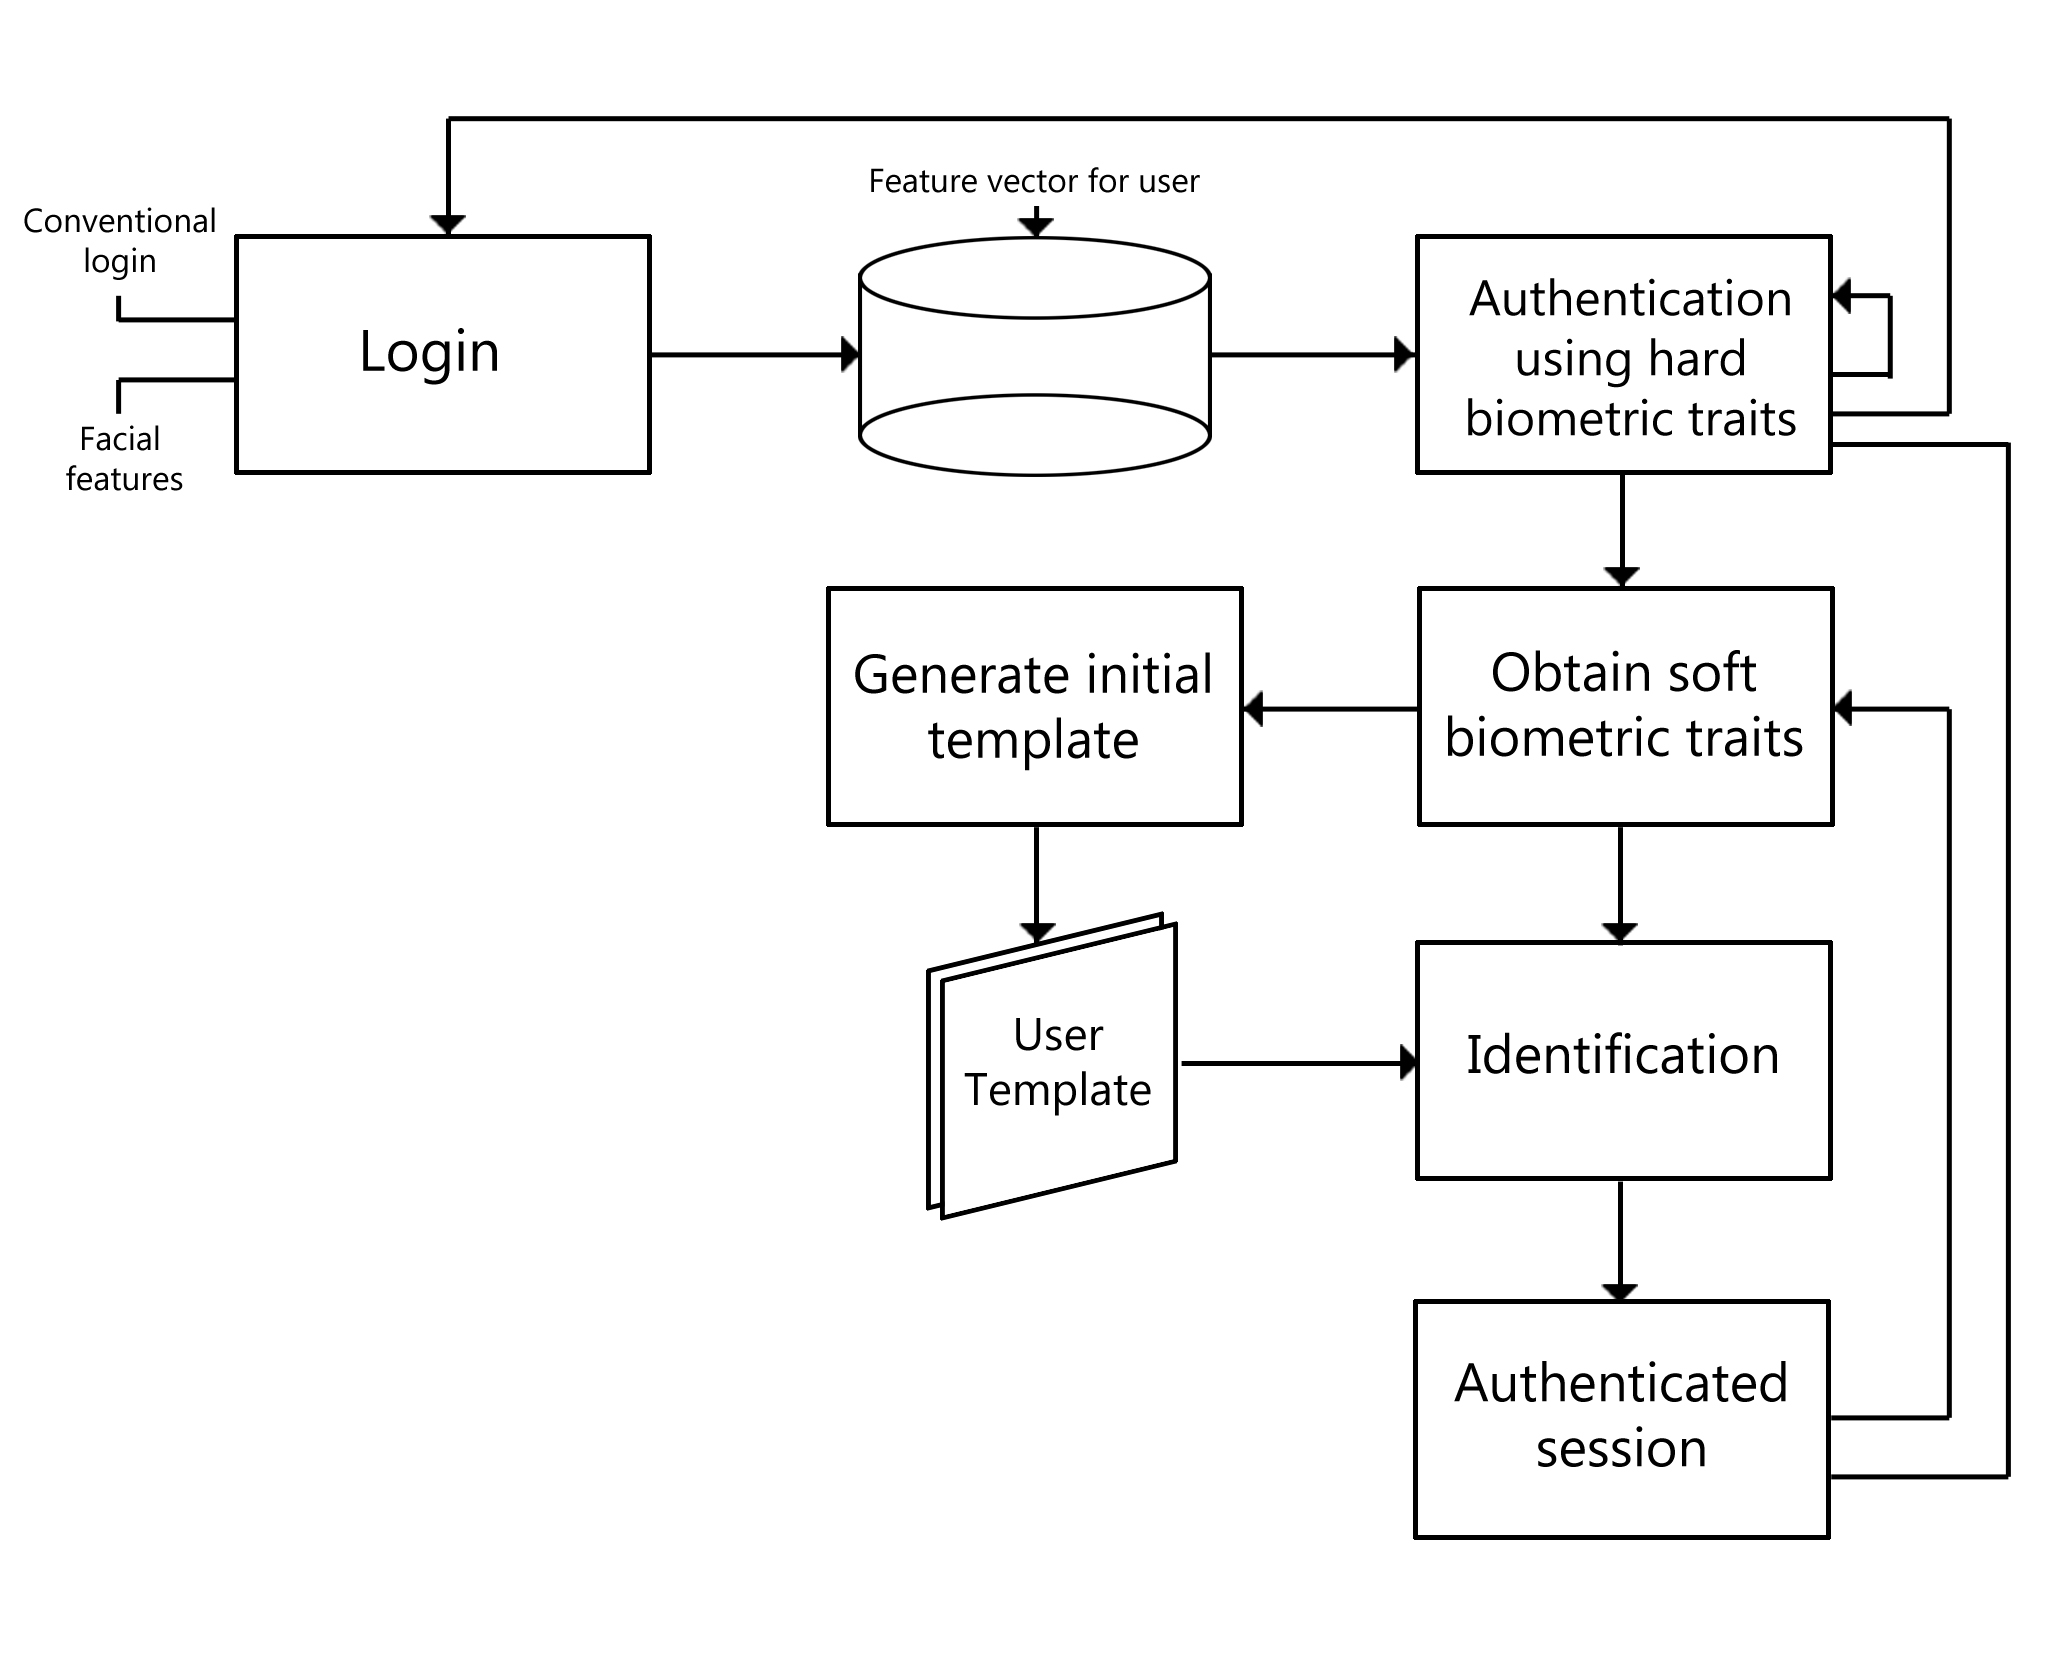
\includegraphics[scale=0.15]{img/auth_overview.jpg}
        \caption{Continuous Authentication System - A Block Diagram.}
        \label{fig:block_diag}
\end{figure}

This system is composed of the following subsystems:
\begin{itemize}
\item Training Subsystem
\item Authentication Subsystem
	\begin{itemize}
	\item Hard Biometric Traits Authentication
	\item Soft Biometric Traits Authentication
	\end{itemize} 
\end{itemize} 

\section {Training Subsystem}
This subsystem is responsible for capturing a new user's facial data and retraining the facial recognition model to incorporate the features of the new user. It can also simply train the model given the training images of all the users. Hence, it consists of two independent modules, namely, account creating module and the training module.
The account creating module asks a user to enter his/her log-in details (username and password) and stores them in an xml file, with the password encrypted by the SHA-1 encryption algorithm. This is followed by capturing a specified number of images of the user's face, which are processed and stored in a specified directory. Then the training module is called, which uses this training set of images to train the face recognition model.
The training module trains the face data so as to implement Eigenfaces, which is the face recognition algorithm employed in our system. In this module, equalized face images of a standard resolution are processed into vector representations. These are combined to form a matrix upon which Principal Component Analysis (PCA) is performed. PCA reduces the dimensionality of the matrix which has a zero empirical mean. This means the that the mean image obtained has been subtracted from each image to obtain the differences. Then a PCA subspace is created with the eachoriginal image being represented as a point in that subspace. This is called "projecting" the training images. Finally, this data is stored as a matrix in an xml file, which can be retrieved later for recognition.
   
\section {Authentication Subsystem}
This subsystem is responsible for authenticating the user, during log-in as well as after that till the session ends. It performs a static authentication when the user is attempting to log-in and if the encrypted password matches, then the Hard Biometric traits authentication starts and performs face recognition of the user. If the user is recognized, then he is successfully logged in. While the user does his work, the face recogniton works continuously in the background to check the facial features of the user. Once a specified level of confidence is achieved, the system transitions to the Soft Biometric traits authentication module. In this mode, the user's shirt colour is stored in a template, and used to continually verify if the shirt is present in the frame. It reverts back to face recognition, if the shirt is not detected in the frame. This system can be further explained by explaining the two phases, namely, Hard Biometric traits authentication and Soft Biometric traits authentication.
 
\subsection{Hard Biometric Traits Authentication}
Hard Biometric Traits refer to the physiological characteristics of a user that uniquely identify that user. These include facial features, fingerprint, iris and others. In our system, we incorporate facial recognition using Eigenfaces. Eigenfaces consists of two parts - training and recognition. The training has been described in the Training Subsystem section above. The recognition occurs as described here. The new face image, captured from the web-cam and processed for Eigenfaces, is projected onto the PCA subspace mentioned in the previous section, and the Euclidian distance is calculated to the closest training image to recognize the user. To improve the accuracy of recognition, a Machine Learning (ML) algorithm is used which studies the confidence value returned by the face recognition algorithm over time and predicts whether the user is actually him/her or an imposter. This ML approach has been implemented by a Support Vector Machine (SVM).

\subsubsection{Face recognition using Eigenfaces}
Eigenfaces are a set of eigenvectors used in the computer vision problem of human face recognition. The approach of using eigenfaces for recognition was developed by Sirovich and Kirby (1987) and used by Matthew Turk and Alex Pentland in face classification. It is considered the first successful example of facial recognition technology. These eigenvectors are derived from the covariance matrix of the probability distribution of the high-dimensional vector space of possible faces of human beings.\\

\subsubsection{ Eigenface generation }
A set of eigenfaces can be generated by performing a mathematical process called principal component analysis (PCA) on a large set of images depicting different human faces. Informally, eigenfaces can be considered a set of "standardized face ingredients", derived from statistical analysis of many pictures of faces. Any human face can be considered to be a combination of these standard faces. For example, one's face might be composed of the average face plus 10\% from eigenface 1, 55\% from eigenface 2, and even -3\% from eigenface 3. Remarkably, it does not take many eigenfaces combined together to achieve a fair approximation of most faces. Also, because a person's face is not recorded by a digital photograph, but instead as just a list of values (one value for each eigenface in the database used), much less space is taken for each person's face.

The eigenfaces that are created will appear as light and dark areas that are arranged in a specific pattern. This pattern is how different features of a face are singled out to be evaluated and scored. There will be a pattern to evaluate symmetry, if there is any style of facial hair, where the hairline is, or evaluate the size of the nose or mouth. Other eigenfaces have patterns that are less simple to identify, and the image of the eigenface may look very little like a face.

The technique used in creating eigenfaces and using them for recognition is also used outside of facial recognition. This technique is also used for handwriting analysis, lip reading, voice recognition, sign language/hand gestures interpretation and medical imaging analysis. Therefore, some do not use the term eigenface, but prefer to use 'eigenimage'.\\[2ex]
{\bf Implementation}\\
To create a set of eigenfaces, one must:
\begin{enumerate}
\item Prepare a training set of face images. The pictures constituting the training set should have been taken under the same lighting conditions, and must be normalized to have the eyes and mouths aligned across all images. They must also be all resampled to a common pixel resolution $(r \times c)$. Each image is treated as one vector, simply by concatenating the rows of pixels in the original image, resulting in a single row with $r \times c$ elements. For this implementation, it is assumed that all images of the training set are stored in a single matrix T, where each row of the matrix is an image.

\item Subtract the mean. The average image a has to be calculated and then subtracted from each original image in T.

\item Calculate the eigenvectors and eigenvalues of the covariance matrix S. Each eigenvector has the same dimensionality (number of components) as the original images, and thus can itself be seen as an image. The eigenvectors of this covariance matrix are therefore called eigenfaces. They are the directions in which the images differ from the mean image. Usually this will be a computationally expensive step (if at all possible), but the practical applicability of eigenfaces stems from the possibility to compute the eigenvectors of S efficiently, without ever computing S explicitly, as detailed below.

\item Choose the principal components. The $D \times D$ covariance matrix will result in D eigenvectors, each representing a direction in the $r \times c$-dimensional image space. The eigenvectors (eigenfaces) with largest associated eigenvalue are kept.
\end{enumerate}
These eigenfaces can now be used to represent both existing and new faces: we can project a new (mean-subtracted) image on the eigenfaces and thereby record how that new face differs from the mean face. The eigenvalues associated with each eigenface represent how much the images in the training set vary from the mean image in that direction. We lose information by projecting the image on a subset of the eigenvectors, but we minimize this loss by keeping those eigenfaces with the largest eigenvalues. For instance, if we are working with a 100 x 100 image, then we will obtain 10,000 eigenvectors. In practical applications, most faces can typically be identified using a projection on between 100 and 150 eigenfaces, so that most of the 10,000 eigenvectors can be discarded.
\noindent{\bf Computing Eigenvectors}
Performing PCA directly on the covariance matrix of the images is often computationally infeasible. If small, say 100 x 100, greyscale images are used, each image is a point in a 10,000-dimensional space and the covariance matrix S is a matrix of 10,000 x 10,000 = 108 elements. However the rank of the covariance matrix is limited by the number of training examples: if there are N training examples, there will be at most N-1 eigenvectors with non-zero eigenvalues. If the number of training examples is smaller than the dimensionality of the images, the principal components can be computed more easily as follows.

Let {\bf T} be the matrix of preprocessed training examples, where each column contains one mean-subtracted image. The covariance matrix can then be computed as {\bf S = T$^{T}$T} and the eigenvector decomposition of {\bf S} is given by\\
\begin{align*}
Sv_{i} = TT^{T}v_{i} = \lambda_{i}v_{i}
\end{align*}
However {\bf T$^{T}$T } is a large matrix, and if instead we take the eigenvalue decomposition of
\begin{align*}
T^{T}Tu_{i} = \lambda_{i}u_{i}
\end{align*}
then we notice that by pre-multiplying both sides of the equation with {\bf T}, we obtain
\begin{align*}
TT^{T}Tu_{i} = \lambda_{i}Tu_{i}
\end{align*}

\subsection{Noise dampening using SVM}
\begin{figure}[h!]
        \begin{subfigure}[b]{0.6\textwidth}
                \centering
                \includegraphics[scale=0.4]{img/wosvm.png}
                \caption{Output of face recognition using Eigenfaces}
                \label{fig:svm1}
        \end{subfigure}%
        \begin{subfigure}[b]{0.5\textwidth}
                \centering
                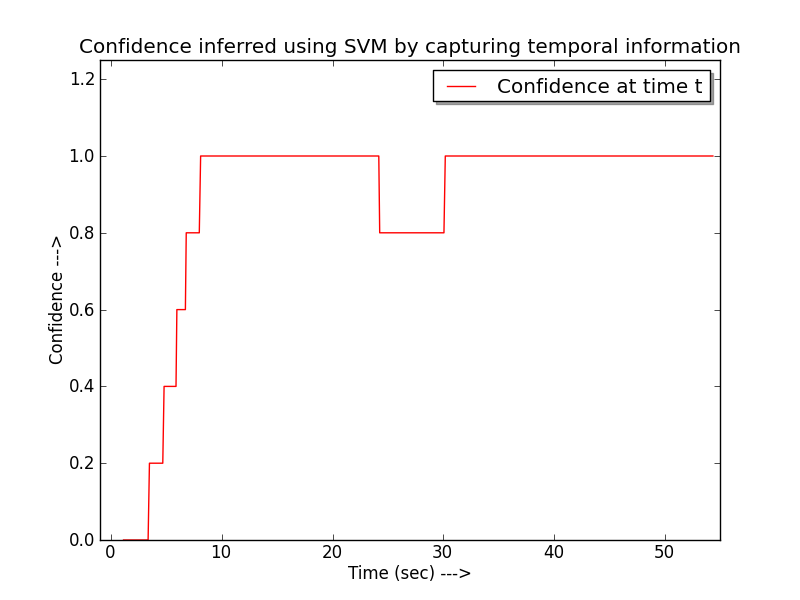
\includegraphics[scale=0.35]{img/svm.png}
                \caption{Used with SVM}
                \label{fig:svm2}
        \end{subfigure}
        \caption{Comparison of systems with/without SVM}\label{fig:pwd}
\end{figure}
The output produced by face recognition using Eigenfaces reflects the nearest neighbour of the projected parameters in the PCA subspace.
The distance is calculated from this projected point to the nearest neighbour in the subspace, using a metric such as Eucledian distance or Mahalanobis distance.
In this project, Mahalanobis distance was used since Euclidean distance doesn't consider scaling factors across dimensions. 
A primitive approach of using \emph{only} output from the face recognition algorithm, raises two issues:
\begin{itemize}
	\item 20-30\% of the output stream produced by the face recognition algorithm is noise, i.e, false negatives.
	\item A person not registered with the database gets recognized as his closest resemblance.
\end{itemize}
To solve these issues, we developed a novel approach using temporal information to predict the authentication state at any given time.
The features used were:
\begin{itemize}
	\item Mean confidence over $X_{t-T}$ to $X_{t}$
	\item Mean time since authentication over $X_{t-T}$ to $X_{t}$
	\item $\sum _{t-T}^{t}\{Recognized\ user = Logged\-in\ user\}$
\end{itemize}
The system was then trained on various cases capturing all instances known, using a classification SVM, with the radial basis function as the kernel.
   
\subsection{Soft Biometric Traits Authentication}
Soft Biometric traits refer to those characteristics of a user that may be behavioural in nature and can identify a user temporarily for a session. In our system, we use the user's colour of clothing as a trait to recognise the user for a session. Once the face recognition achieves a sufficiently high level, the shirt detection module begins. Over a few frames, it collects information about the user's shirt colour. This works by detecting a face in the frame and then checking for the colour in a rectangular region at an appropriate distance below the face. The colour information is stored in a template and is used to match the colour information obtained in the future frames with it. If an anomaly is detected, as in, the user's face is not detected (for the case where a user has moved away from the system temporarily) or a different colour is detected (for the case where an unauthorized user has quickly appeared in the frame in the absence of the actual user), then facial recognition is restarted to check for the authentic user.
\end{document}
